\chapter{Marktanalyse} \label{Marktanalyse}

Wie schon in der Anforderungsanalyse (Kapitel \ref{Anforderungsanalyse}) beschrieben, werden die 3 aktuell relevantesten Frameworks für hybride, bzw. Cross-Platform-Anwendungsentwicklung ausgewählt, um diese mit einer Funktionstest-Anwendung zu evaluieren.
\\
\\
Bevor eine allgemeine Liste aktuell verfügbarer Frameworks aufgestellt wurde, wurden folgende Kriterien festgelegt, welche auf jeden Fall von den Frameworks erfüllt werden müssen, um bei dieser Evaluation Berücksichtigung zu finden: Die Frameworks müssen mehr als eine Plattform bedienen, und 2 dieser Plattformen müssen Android und iOS sein, da diese den größten Marktanteil besitzen (siehe Kapitel \ref{Einleitung}). Wobei Android einen durchschnittlichen Marktanteil von ca. 75\% und iOS von ca. 18\% über die vergangenen 4 Jahre besaß\footcite{Statista}.
Folgende Frameworks konnten nach oben genannten Kriterien ausfindig gemacht werden:
\\
\begin{itemize}
\item React Native
\item CodenameOne
\item Xamarin
\item Ionic
\item Intel XDK
\item Onsen UI
\item Kendo UI
\item Mobile Angular UI
\item Cordova
\item PhoneGap
\item J2ObjC
\item AppGyver
\item ViziApps
\item Monocross
\item Marmalade
\item Corona
\item Agate
\item Apache Flex
\item AppConKit
\end{itemize}

Um die 3 aktuell relevantesten Frameworks zu ermitteln, wurden folgende Medien genutzt: Mit dem Google AdWords Keyword Planer\footcite{KeyWordPlaner} wurden die durchschnittlichen Suchanfragen nach dem Namen des jeweiligen Frameworks pro Monat über den Zeitraum des letzten Jahres ermittelt. Hierbei ergab sich bei den oben aufgeführten Frameworks folgende Verteilung:
\clearpage
\begin{figure}[h]
	\centering
	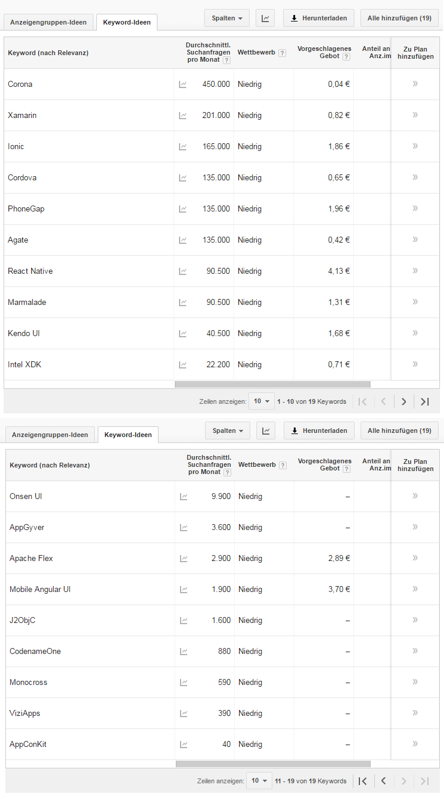
\includegraphics[width=0.6\textwidth]{Bilder/Durchschnittliche_Suchanfragen_gesamt.PNG}
	\caption{Durchschnittliche Suchanfragen bei Google, ermittelt mit Google AdWords Keyword Planer}
	\label{fig:Suchanfragen1}
\end{figure}

\clearpage
Zusätzlich wurden mit Hilfe von Google Trends\footcite{GoogleTrends} die Popularität der einzelnen Frameworks im Zeitverlauf visualisiert, um zu verdeutlichen welche Frameworks in letzter Zeit an Interresierten dazugewonnen haben. Die Ergebnisse werden bei Google Trends in Relation zum totalen Suchaufkommen gesetzt. Die Trends sind für einzelne Regionen sowie für die ganze Welt verfügbar. In diesem Fall wurden die weltweiten Trends für die Frameworks ausgewertet. Da sich nur 5 Suchbegriffe gleichzeitig in einem Graphen gegenüberstellen lassen, wurden immer 4 Frameworks 'Corona', welches in der vorherigen Untersuchung mit dem Keyword Planer\footcite{KeyWordPlaner} die meisten monatlichen Suchanfragen aufwies, als Referenz gegenübergestellt. Da einige Frameworks Namen haben, die auch in völlig anderen Zusammenhängen gesucht werden können, wie zum Beispiel 'Marmalade', wurde als Suchkategorie 'Computer und Elektronik' ausgewählt.
\\
\\
\begin{figure}[h]
	\centering
	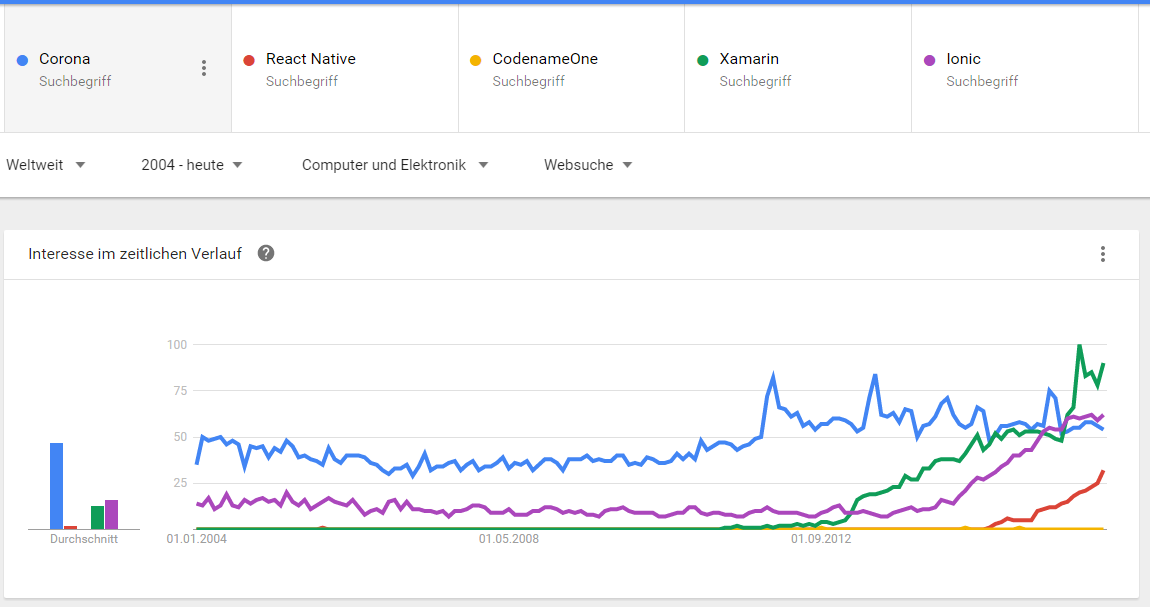
\includegraphics[width=0.8\textwidth]{Bilder/trends_1.PNG}
	\caption{Google Trends: React Native, CodenameOne, Xamarin und Ionic im Vergleich zu Corona}
	\label{fig:Trends1}
\end{figure}
\begin{figure}[h]
	\centering
	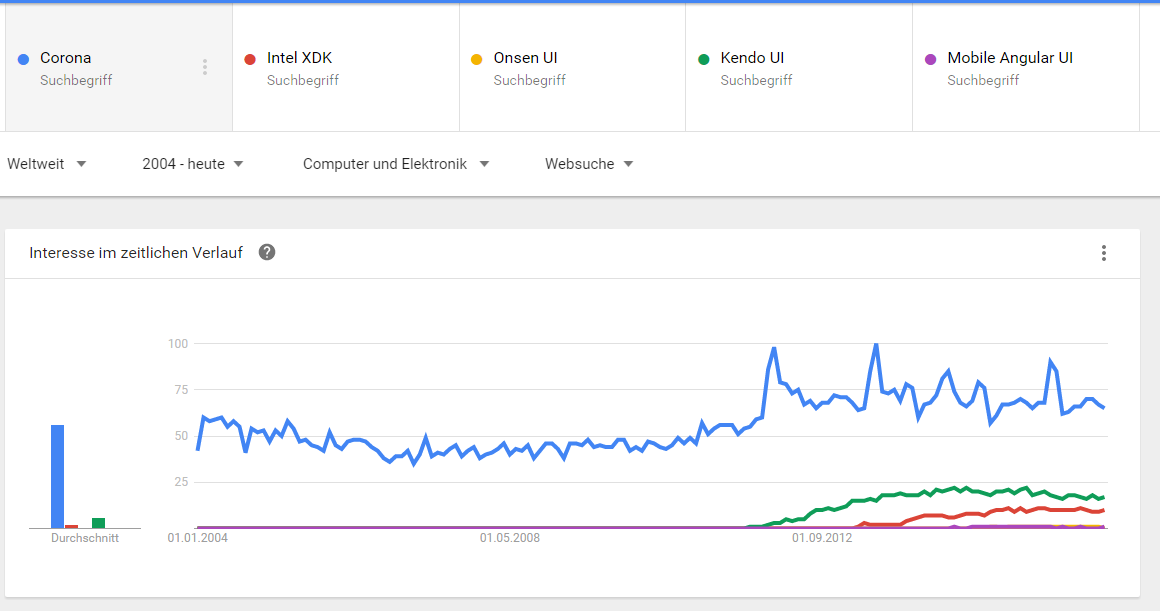
\includegraphics[width=0.8\textwidth]{Bilder/trends_2.PNG}
	\caption{Google Trends: Intel XDK, Onsen UI, Kendo UI und Mobile Angular UI im Vergleich zu Corona}
	\label{fig:Trends2}
\end{figure}
\begin{figure}[h]
	\centering
	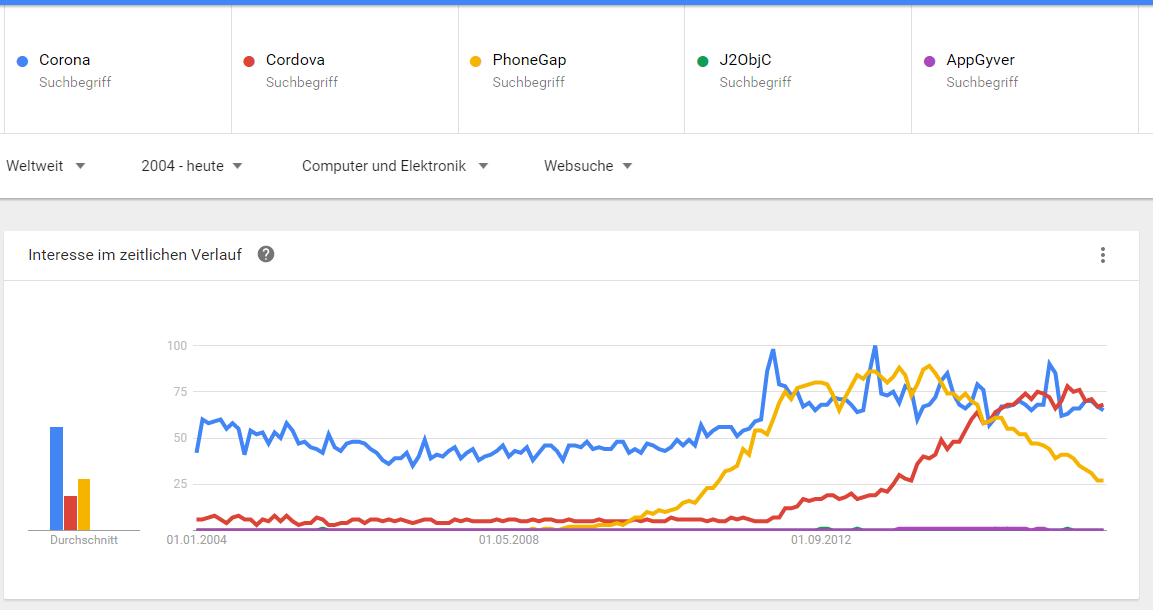
\includegraphics[width=0.8\textwidth]{Bilder/trends_3.PNG}
	\caption{Google Trends: Cordova, PhoneGap, J2ObjC und AppGyver im Vergleich zu Corona}
	\label{fig:Trends3}
\end{figure}
\begin{figure}[h]
	\centering
	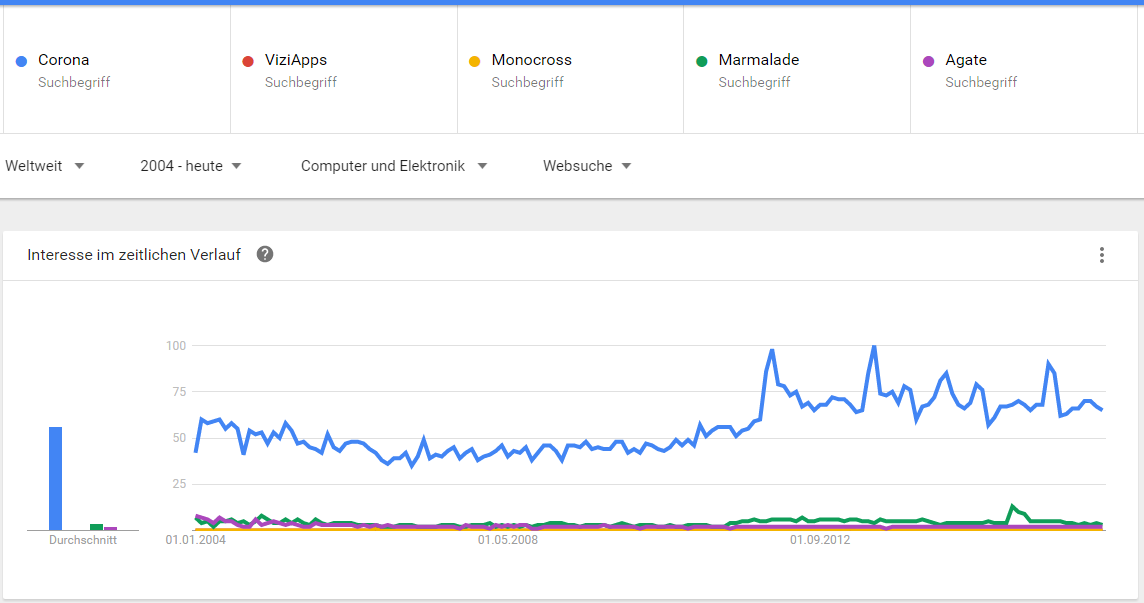
\includegraphics[width=0.8\textwidth]{Bilder/trends_4.PNG}
	\caption{Google Trends: ViziApps, Monocross, Marmalade und Agate im Vergleich zu Corona}
	\label{fig:Trends4}
\end{figure}
\begin{figure}[h]
	\centering
	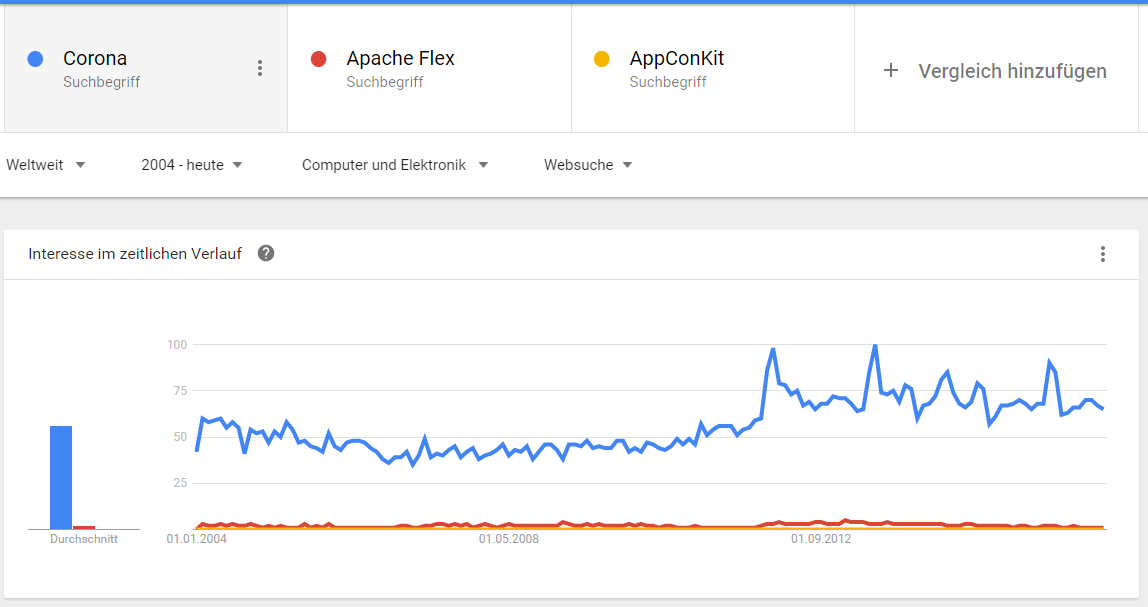
\includegraphics[width=0.8\textwidth]{Bilder/trends_5.PNG}
	\caption{Google Trends: Apache Flex und AppConKit im Vergleich zu Corona}
	\label{fig:Trends5}
\end{figure}
\clearpage
Aus oben beschriebenen und dargestellten Auswertungen ergeben sich zunächst folgende 5 Frameworks in der engeren Auswahl, welche durch die Implementierung einer Funktionstest-Anwendung evaluiert werden sollen:
\begin{itemize}
\item Corona
\item Xamarin
\item Cordova
\item PhoneGap
\item Ionic
\end{itemize}
Aufgrund der vergleichsweise sehr geringen Repräsentation des Frameworks Corona auf GitHub (ca. 2000 Repositories im Vergleich zu um die ca. 30.000 Einträge zu Ionic oder React Native) wird dieses von den oben aufgelisteten Frameworks hintenangestellt\footcite{GitHubTrending}. Nach weiteren Recherchen über diese 5 Frameworks stellte sich noch heraus, dass es sich bei Cordova um eine Weiterentwicklung des Frameworks PhoneGap handelt. Dies schlägt sich auch in den Google Trends nieder, wie man in Abbildung \ref{fig:Trends3} erkennen kann. Aus diesem Grund wird ausschließlich Cordova evaluiert, der Vorgänger PhoneGap bleibt außen vor. Für die Liste der zu evaluierenden Frameworks ergibt sich daraus, dass an die Stelle von PhoneGap nun 'React Native' tritt. 
\\
\\
Das Framework Cordova bietet keine Mittel für die Realisierung einer grafischen Benutzeroberfläche und für das Framework Ionic ist für sämtliche Hardware-Nutzung das Einbinden von Cordova-Plugins notwendig. Aus diesen Gründen werden diese beiden Frameworks in dieser Arbeit kombiniert betrachtet, als 2 Bausteine eines Frameworks sozusagen. So ergeben sich für die Evaluation in dieser Arbeit die Frameworks Xamarin, React Native und Cordova mit Ionic. Diese Frameworks werden nachfolgend etwas näher vorgestellt. 

\section{Xamarin} \label{chpXamarin}

Das Xamarin Framework verspricht native Anwendungen für Windows Phone, iOS und Android entwickeln zu können basierend auf einer C\# Codebase. Konkret gesprochen verspricht es eine native UI, nativen API Zugang und native Performance Xamarin kommt mit der eigenen IDE 'Xamarin Studio', es ist allerdings auch möglich Xamarin Anwendungen mit der IDE 'Visual Studio' zu entwickeln. Die Benutzeroberfläche muss bei Xamarin Anwendungen allerdings für jede Plattform separat implementiert werden\footcite{EinerFuerAlles}. 

\section{Cordova} \label{chpCordova}

Cordova von Apache ist ein Open Source Framework für Cross-Platform mobile Anwendungsenwicklung. Das Framework ist kostenlos nutzbar und unterstützt Standard Web Technologien wie HTML5, CSS3 und JavaScript für die Entwicklung. Die Anwendungen werden in sogenannten Wrappern ausgeführt, die die API der jeweiligen Plattform ansprechen um so Zugang zu unter anderem Sensoren zu bekommen. Die Plattformen, die von Apache Cordova unterstützt werden sind: Android, Blackberry 10, iOS, OS X, Ubuntu, Windows und Windows Phone 8\footcite{Cordova}. 

\section{Ionic}

Das Ionic Framework basiert auf AngularJS, was wiederum ein clientseitiges JavaScript-Webframework ist\footcite{AngularJS}. Entsprechend werden Ionic Anwendungen ebenfalls in JavaScript, HTML5 und CSS3 geschrieben. Auf diese Weise wird bei diesem Framework die gemeinsame Code-Basis geschaffen. Ionic bietet eine nativ wirkende GUI, für Hardware-Anbindungen, wie zum Beispiel das Nutzen von Sensoren, müssen allerdings Cordova (Kapitel  \ref{chpCordova}) PlugIns genutzt werden\footcite{Ionic}. 

\section{React Native}

React Native nutzt die Bibliothek React von Facebook zur Entwicklung für die Plattformen Android, iOS und die Universal Windows Platform. Programmiert werden React Native Anwendungen in JavaScript und HTML. Der Code wird anschließend in native Quelldateien übersetzt, weshalb React Native verspricht native Komponenten ohne großen Aufwand einbinden zu können und flüssige Animationen zu ermöglichen\footcite{EinerFuerAlles}.